\chapter{Konzept und Architektur}
scalierbarkeit wieso man es braucht für das projekt?

In diesem Kapitel wird das konzeptionelle und technische Fundament des entwickelten Systems beschrieben. 
Ziel ist es, eine skalierbare, fehlertolerante und reaktive Architektur zu realisieren, die sowohl Live-Daten 
als auch historische Daten effizient verarbeiten kann. Diese Daten werden in das System integriert, verwaltet 
und so aufbereitet, dass sie für nachgelagerte Komponenten leicht zugänglich und weiterverarbeitbar sind. 
Im weiteren Verlauf werden zunächst die Grundlagen der Skalierbarkeit erläutert, bevor die Systemarchitektur, 
die Rollen der Cluster-Komponenten sowie die Kommunikations- und Datenflüsse innerhalb des Systems vorgestellt 
werden.

\section{Skalierbarkeit und Motivation}

Ein zentraler Aspekt des Projekts ist die effiziente Verarbeitung großer Datenmengen in Echtzeit. 
Im Kontext der Formel-1-Datenanalyse entstehen pro Rennen mehrere hunderttausend Datensätze, 
die eine Vielzahl unterschiedlicher Informationen umfassen, von Telemetriedaten über Zwischenzeiten, 
Positionswechsel und Boxenstopps bis hin zu Sektorzeiten. Diese Datenströme sollen parallel verarbeitet 
und in aggregierter Form zur Darstellung der aktuellen Rennsituation der einzelnen Fahrer bereitgestellt werden.

Um sicherzustellen, dass das System auch bei steigender Datenrate zuverlässig arbeitet, muss es skalierbar ausgelegt sein. 
Skalierbarkeit beschreibt die Fähigkeit eines Softwaresystems, seine Leistungsfähigkeit durch das Hinzufügen von Ressourcen zu erhöhen, 
ohne Änderungen an der Anwendung selbst vornehmen zu müssen \parencite{bass2021}. Ein skalierbares System kann 
somit wachsende Datenmengen oder Benutzeranforderungen verarbeiten, ohne dass ein vollständiges Redesign erforderlich wird.

Im Rahmen dieses Projekts wird eine horizontale Skalierung realisiert. 
Die Anwendung kann als verteiltes System mit mehreren Knoten betrieben werden, 
wobei die einzelnen Rollen des Systems entweder gemeinsam in einem Prozess oder getrennt auf unterschiedliche 
Knoten verteilt ausgeführt werden können. Diese flexible Ausführungsstrategie ermöglicht sowohl den Betrieb 
als monolithische Anwendung als auch eine skalierte Ausführung über mehrere Prozesse oder physische Maschinen. 
Selbst im monolithischen Modus kann das System dynamisch erweitert werden, indem zusätzliche Prozesse 
in den Cluster eingebunden werden. Durch das Hinzufügen weiterer Knoten wird die Arbeitslast automatisch auf 
mehrere Instanzen verteilt, was sowohl die Gesamtleistung als auch die Fehlertoleranz erhöht. 
Fällt ein Knoten aus, übernehmen verbleibende Instanzen mit derselben Rolle automatisch deren Aufgaben.

Durch den Einsatz von Akka.NET und dem Cluster Sharding Mechanismus 
können neue Knoten nach ihrer Registrierung am Hauptknoten dynamisch in das System integriert werden. 
Nach dem Beitritt zum Cluster übernehmen sie automatisch Teile der Verarbeitung, 
ohne dass Konfigurationsänderungen oder Neustarts erforderlich sind \parencite{akkaNet}.
Dieses Skalierungsprinzip führt zu einer flexiblen und anpassungsfähigen Architektur,
bei der neu hinzukommende Prozesse automatisch in den Cluster integriert werden,
ohne dass zusätzliche Konfigurationsschritte erforderlich sind.

\section{Gesamtarchitektur des Systems}
Die Architektur des entwickelten Systems basiert auf dem Akka.NET-Framework und nutzt dessen Cluster-Mechanismen zur Realisierung einer verteilten, fehlertoleranten und skalierbaren Anwendung.
Abbildung "architecture-diagramm" zeigt die zentralen Komponenten des Systems und deren Interaktion.
%\ref{fig:architecture} #architecture-diagramm#
% \begin{figure}[H]
%     \centering
%     \includegraphics[width=0.8\textwidth]{images/architecture_diagram.png}
%     \caption{Architekturübersicht des verteilten Systems}
%     \label{fig:architecture}
% \end{figure}
Das System besteht aus mehreren Knoten, die unterschiedliche Rollen übernehmen. Für den Betrieb des Clusters sind grundsätzlich zwei Ausführungsmodi vorgesehen:
\begin{itemize}
    \item \textbf{Monolithischer Modus:} 
    In diesem Modus werden alle Rollen innerhalb eines einzelnen Prozesses ausgeführt.
    Diese Variante eignet sich insbesondere für Entwicklungs- und Testzwecke, da sie die Systemkomplexität 
    reduziert und die Einrichtung vereinfacht.
    \item \textbf{Verteilte Ausführung:} 
    Hierbei werden die verschiedenen Rollen auf separate Prozesse oder physische Maschinen verteilt.  
    Dadurch wird eine effizientere Ressourcennutzung ermöglicht und das System kann bei steigender Last 
    horizontal skaliert werden, da einzelne Komponenten unabhängig voneinander erweitert werden können.
\end{itemize}

Jeder Knoten im Cluster kann eine der folgenden Rollen übernehmen: Ingress, Backend und Coordinator.
Diese Rollen sind für die verschiedenen Aufgaben innerhalb des Systems verantwortlich und arbeiten zusammen, um die Verarbeitung und Bereitstellung der Daten sicherzustellen.

Zur Verwaltung und strukturierten Weiterleitung der Daten wird das Cluster-Sharding-Konzept von Akka.NET eingesetzt.
Damit Nachrichten effizient an die jeweilige ShardRegion gesendet und von dieser empfangen werden können, kommen Proxies zum Einsatz, die als Vermittler zwischen den Knoten und den Shards fungieren.

Ein integrierter Load Balancer verteilt eingehende Datenströme aus externen Quellen gleichmäßig auf mehrere Arbeitsknoten.
Diese Knoten leiten die empfangenen Daten anschließend an die zuständige ShardRegion weiter, wo sie verarbeitet und persistiert werden.

Um die Kommunikation zwischen den verteilten Komponenten sicherzustellen, wird zudem ein verteiltes Publish/Subscribe-System eingesetzt.
Dieses ermöglicht es den verschiedenen Rollen, Nachrichten asynchron auszutauschen und auf Ereignisse zu reagieren, ohne dass direkte Verbindungen erforderlich sind.


\section{Rollen im Cluster}

Dieses Kapitel beschreibt die drei Hauptrollen innerhalb des Clusters: Ingress, Backend und Coordinator.
Jede dieser Rollen erfüllt eine klar abgegrenzte Funktionalität und trägt gemeinsam zur Gesamtfunktionalität des Systems bei.

\subsection{Ingress}

Der Ingress-Knoten ist für die Datenbeschaffung und -weiterleitung an die ShardRegion zuständig.
Die Kommunikation erfolgt über Proxies, die als Vermittler zwischen den eingehenden Datenströmen und den zuständigen Shards fungieren.

Zur Steuerung des Datenflusses wird Akka.Streams verwendet, wodurch eingehende Datenströme effizient verarbeitet werden können.
Bei hohen Datenmengen sorgen integrierte Backpressure-Mechanismen dafür, dass keine Überlastung der Arbeitsknoten entsteht.
Um Datenverluste zu vermeiden, sendet der Ingress-Knoten neue Daten erst dann an die Arbeitsknoten weiter, wenn eine Bestätigung der ShardRegion vorliegt.
Dies gewährleistet eine kontrollierte und zuverlässige Datenaufnahme innerhalb des Clusters.

\subsection{Backend}

Der Backend-Knoten ist für die eigentliche Verarbeitung und Speicherung der eingehenden Daten verantwortlich.
Er empfängt die Daten vom Ingress-Knoten und speichert sie in einer Datenstruktur, die als Modell für die Formel-1-Daten dient.
Nach erfolgreicher Verarbeitung und Speicherung werden die aufbereiteten Daten über einen sogenannten Händler-Knoten an die entsprechenden Konsumenten weitergeleitet.

Zur Sicherstellung der Datenpersistenz werden die Informationen entweder in einer In-Memory-Datenbank oder einer PostgreSQL-Datenbank abgelegt.
Um Datenverluste bei Ausfällen oder Neuzuweisungen von Backends zu verhindern, kommt die Akka.Persistence-Funktionalität zum Einsatz.
Dabei werden regelmäßig sogenannte Snapshots erstellt, anstatt jede einzelne Änderung sofort zu speichern.
Dies reduziert die Datenbanklast und gewährleistet gleichzeitig eine schnelle Wiederherstellung.

Nach einem Neustart oder einem Failover kann der aktuelle Zustand durch das Wiederherstellen der gespeicherten Snapshots und das erneute Abspielen der nachfolgenden Events rekonstruiert werden.

\subsection{Coordinator}

Der Coordinator-Knoten übernimmt die Verwaltung und Überwachung des Clusters.
Er stellt sicher, dass die verschiedenen Komponenten reibungslos zusammenarbeiten und auf neu beitretende oder ausgefallene Knoten korrekt reagieren.

Eine zentrale Aufgabe des Coordinators besteht darin, den Zustand der ShardRegion zu überwachen.
Falls keine funktionsfähige Region verfügbar ist, beispielsweise nach einem Node-Ausfall oder während einer Rebalancing-Phase, verhindert der Coordinator, dass der Ingress-Knoten weiterhin Daten an die ShardRegion sendet.
Er fungiert somit als Kontrollinstanz, die sicherstellt, dass Daten nur dann in den Cluster eingespeist werden, wenn eine stabile und empfangsbereite Verarbeitungseinheit vorhanden ist.

Darüber hinaus übernimmt der Coordinator allgemeine Verwaltungs- und Überwachungsaufgaben, wie das Erfassen von Clusterstatusmeldungen oder das Weiterleiten relevanter Ereignisse an andere Komponenten.

\section{Cluster Sharding}

Cluster Sharding ist ein Mechanismus, der es Cluster-Akteuren ermöglicht, über ihre logischen IDs zu kommunizieren, ohne die physischen Standorte der Zielakteure kennen zu müssen \parencite{getakka_cluster_sharding}.  
Es handelt sich um ein Werkzeug, das die verteilte Verwaltung zustandsbehafteter Akteure über mehrere Knoten innerhalb eines Clusters ermöglicht \parencite{cluster_sharding_petabridge}.  

Der strukturelle Aufbau des Cluster Shardings ist wie folgt gegliedert:

\begin{figure}[H]
    \centering
    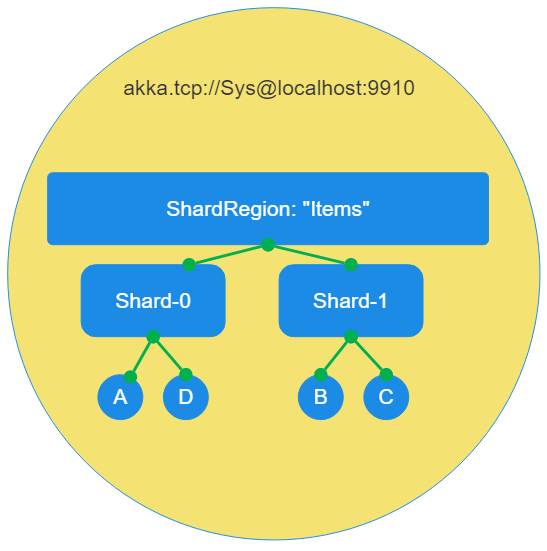
\includegraphics[width=0.5\textwidth]{assets/cluster-sharding.png}
    \caption{Cluster Sharding Architektur \parencite{cluster_sharding_petabridge}}
    \label{fig:architecture}
\end{figure}

\begin{itemize}
    \item \textbf{ShardRegion:}
    Eine logische Gruppierung von Entitäten, die über mehrere Knoten im Cluster verteilt sind. Sie dient als zentraler Einstiegspunkt für eingehende Nachrichten und verwaltet die Zuordnung von Shards zu den entsprechenden Knoten \parencite{cluster_sharding_petabridge}.
    \item \textbf{Shard:}
    Die eigentliche Verteilungseinheit, die festlegt, auf welchem Clusterknoten sich eine Gruppe von Entitäten befindet. Intern fungiert sie als übergeordneter Akteur für ihre Entitäten im Sinne des Child-per-Entity-Musters \parencite{cluster_sharding_petabridge}.
    \item \textbf{Entity:}
    Die kleinste Einheit im Cluster Sharding. Eine Entität repräsentiert einen konkreten, zustandsbehafteten Akteur, der über eine eindeutige ID identifiziert wird und eigenständig Nachrichten empfangen sowie verarbeiten kann \parencite{cluster_sharding_petabridge}.
\end{itemize}

Das Ziel des Cluster Shardings besteht darin, sicherzustellen, dass im gesamten Cluster stets genau eine Instanz jeder Entität existiert.  
Darüber hinaus wird eine gleichmäßige Verteilung der Entitäten über alle verfügbaren Knoten angestrebt, um eine optimale Ressourcenauslastung und Lastverteilung zu gewährleisten.  
Dies wird durch den Einsatz von Hashing-Algorithmen erreicht, die bestimmen, auf welchem Knoten eine bestimmte Entität platziert wird.  

Die ShardRegion ist zudem für das Rebalancing verantwortlich, also die Umverteilung von Shards, wenn Knoten dem Cluster beitreten oder diesen verlassen.  
Darüber hinaus koordiniert sie den Lebenszyklus der Entitäten, indem sie diese bei Bedarf erstellt, passiviert oder entfernt \parencite{cluster_sharding_petabridge}.

\subsection{Neuausgleich der Shards}

Ein zentraler Aspekt des Cluster Shardings ist der Neuausgleich (Rebalancing) der Shards.  
Dieser Prozess wird vom Shard-Koordinator gesteuert, der alle beteiligten Akteure im Cluster darüber informiert, dass die Übergabe einer Shard begonnen hat.  
Zunächst werden alle eingehenden Nachrichten für die betroffene Shard zwischengespeichert, bis die Übergabe abgeschlossen ist.  
Sobald die Übertragung abgeschlossen ist, werden die alten Shard-Instanzen beendet und die zwischengespeicherten Nachrichten an die neuen Shard-Instanzen weitergeleitet \parencite{cluster_sharding_petabridge}.  

Während dieses Prozesses wird der Zustand der Entitäten nicht direkt migriert.  
Um Datenverlust zu vermeiden, sollten Entitäten daher so gestaltet sein, dass sie ihren Zustand persistent speichern können \parencite{cluster_sharding_petabridge}.  

Die Logik für das Rebalancing kann bei Bedarf durch die Implementierung einer benutzerdefinierten Zuweisungsstrategie angepasst werden.  
Standardmäßig verwendet Akka.NET eine Hash-basierte Zuweisungsstrategie, die eine gleichmäßige Verteilung der Shards über die verfügbaren Clusterknoten sicherstellt \parencite{getakka_cluster_sharding}.

\subsection{ShardRegion-Proxy}


Ein ShardRegion-Proxy wird benötigt, wenn eine Kommunikation mit einer ShardRegion stattfindet, die sich nicht auf demselben Knoten befindet\parencite{getakka_cluster_sharding}.

Da die ShardRegion-Instanz ausschließlich auf den Knoten mit der Rolle \textit{Backend} existiert, muss ein Proxy verwendet werden, um von außerhalb dieser Rolle auf die ShardRegion zuzugreifen.

\section{Singleton}




\subsection{Singleton-Proxy}

\section{Kommunikation über Verteiltes Pub/Sub}

\section{Streams}

\subsection{Overflowstrategien}


\section{Alternative Architekturvarianten}
